\subsubsection*{Methodology of the IMG subproject}


\begin{figure}[!htb]
	\centering
	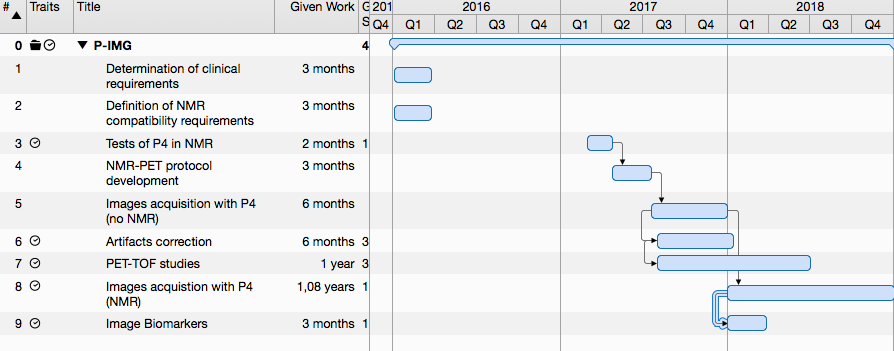
\includegraphics[scale=0.5]{img/ImgWF.png}
	\caption{\label{fig.ImgWF} Work flow for the activities of the IMG subproject.  }
\end{figure}

\paragraph{Definition of clinical requirements:}

In the very process of the PET device development some clinical requirement should be reached for an accurate spatial and temporal resolution. This requirements would be reviewed and studied from the existing literature and the state of the art.

Also, as the integration of both system will be performed in the La Fe Hospital installations, different compatibility prerequisite between PET and NMR will be evaluated to be considered in the PET development. Namely:
\begin{itemize}
\item The influence of the magnetic field on the new detectors developed. PETALO will be combined with a 3T (127Mhz) NMR device.
\item The size of the gantry of the NMR device, which is 60 cm.
\item The building materials of the PET device, which are meant to be adequate to avoid or have minimal artefacts in NMR images. 
\end{itemize}

\paragraph{NMR images acquisition}

In the final phase of prototype integration it will be necessary to test the compatibility of PETALO with the NMR system by performing several studies. These exams will comprise the development of protocols (sequences to be specified) for the acquisition of images with combined NMR and PET data and the storage of the images acquired into the hospital PACS

\paragraph{Integration of imaging biomarkers in the workflow}

The NMR-PET system will include the automated generation of imaging biomarkers derived from the acquisition profiles and sequences considered, like Pharmacokinetics imaging biomarkers extracted from MR Perfusion acquisitions (like vascular permeability, Ktrans; extraction rate, Kep; extra-vascular extra-cellular volume, ve) and also MR Diffusion (like apparent diffusion coefficient, ADC; and diffusion coefficient, D; pseudo-diffusion or perfusion coefficient, D*; vascular fraction, f). The automated quantification of the Metabolic Activity through the standardized uptake value (SUV) in the clusters with higher SUV values will be also developed\footnote{Ralf S. Eschbach , Wolfgang P. Fendler , Philipp M. Kazmierczak,, Marcus Hacker, Axel Rominger , Janette Carlsen , Heidrun Hirner-Eppeneder , Jessica Schuster , Matthias Moser , Lukas Havla , Moritz J. Schneider , Michael Ingrisch , Lukas Spaeth , Maximilian F. Reiser , Konstantin Nikolaou , Clemens C. Cyran Correlation of Perfusion MRI and 18F-FDG PET Imaging Biomarkers for Monitoring Regorafenib Therapy in Experimental Colon Carcinomas with Immunohistochemical Validation. PLoS One. 2015; 10(2): e0115543.}.

\paragraph{Testing the compatibility of P4 with NMR}
According to the schedule of the DET subproject, P4 will be built and characterised by Q4-16. In Q1-217 the detector will be installed inside the gantry of the NMR research apparatus available at the hospital La Fe (a 3T, 127Mhz apparatus with a 60 cm gantry). This is an essential test for the certification of PETALO as a fully compatible NMR apparatus. The compatibility requirements between NMR magnetic fields and P4 will be evaluated studying the influence of the magnetic field on the building materials, the sensors and ---as soon as available--- the (first stage) PETALO APE. The tests will run  through Q1-2017 and will include studies of combined PET and NMR data. 

\paragraph{Definition of clinical requirements and certification of P4}
During Q2-17, the quality and safety requirements to be used in a clinical environment will be defined, so that the system can be certified for operation at La Fe in Q2-17.

\paragraph{Study and modelling of image degradation phenomena for P4}

Like any PET device, PETALO will need a deep study to understand the  
degradation processes that affect the final determination of the images\footnote{Sune H. Keller,  Søren Holm, Adam E. Hansen, Bernhard Sattler, Flemming Andersen, Thomas L. Klausen, Liselotte Hojgaard,  Andreas Kjær, Thomas Beyer. Image artifacts from MR-based attenuation correction in clinical, whole-body PET/MRI. Magn Reson Mater Phy (2013) 26:173–181}. There are a number of them which will be of capital importance such as random coincidences, order of the sequence of the interactions, missing projection data, continuous energy spectrum of the gamma prompts, etc. These effects will be accurately modelled in order to minimise the negative impact in the imaging.

Most of these processes can be compensated at reconstruction time by computing a system matrix (SM) modelling the whole device. Other corrections can be added at hoc. However, the excellent timing and energy resolution expected for PETALO will likely a very well behaved SM. 

In summary, a dedicated image reconstruction software package for P4 will be developed. It should be flexible enough to accommodate many possible configurations. The device will be modelled with high degree of precision for achieving final images of the highest possible quality. 

According to the schedule P4 will be available in Q2-2017 for imaging studies after a full characterisation of its operational parameters (energy resolution, spatial resolution, CRT). The detector will then be operated for at least six months (Q3/Q4-17) as an imaging device (without magnetic fields) using phantoms and small animals to compute the SM and develop the imaging software.  

\paragraph{TOF imaging}

For image reconstruction, the Maximum Likelihood Estimation Maximization
(MLEM) is a commonly used method for PET and provides the possibility to include
Time-Of-Flight (TOF) information\footnote{Groiselle C J and Glick S J (2004): 3D PET list-mode iterative reconstruction using time-of-flight
information. IEEE Nucl. Sci. Symp. Conf. Record 2633-2638.}. The improvement in image quality achieved by TOF-MLEM reconstruction compared with standard MLEM for PET strongly depends
on the time resolution of the scanner. Currently, for commercially available crystal-based PET scanners the best coincidence resolving time (CRT) is currently   500-600 ps FWHM. As an example, the Philips Gemini TF made of LYSO and used for diagnostic PET shows 585 ps FWHM CRT\footnote{Surti S, Kuhn A, Werner M E, Perkins A E, Kolthammer J, and Karp J S (2007): Performance of
Philipps Gemini TF PET/CT Scanner with Special Consideration for Its Time-of-Flight Imaging
Capabilities. J Nucl Med 48 471-48}.
Recently, a new generation of PET scanners based on silicon photomultiplier provides
CRTs of 400 ps, as referenced in manufacturer data sheets (Philips Vereos PET/CT and
GE Signa PET/MR).

The IMG and the DET group will develop the TOF-MLEM reconstruction jointly to take advantage of the excellent CRT resolution expected for PETALO ($\sim 200-250$~ps), which would be, if confirmed, the best in the market. 

\paragraph{Acquisition of images with combined MR and PET data}
In 2018, P4 will operate inside the NMR gantry. 
The software for registration and fusion of the MR and PET images will be developed considering different techniques (segmentation, atlas-based) for the generation of attenuation maps in the PET images correction. Operation in the presence of magnetic field will run from Q1 to Q4 2018. The combination of the excellent energy and time resolution, TOF capabilities and NMR combined images should provide a strong demonstration of the strength of the technology. 

